%!Tex engine = XeLaTeX
\documentclass[10pt]{beamer}
%,aspectratio=169 %画面比例16:9
\usepackage{XDstyle}
%\usepackage[English,CircleLogo,XDblue]{XDstyle}


\title{这是标题Title}
\subtitle{子标题}
\institute{西安电子科技大学~数学与统计学院\\邮箱:$\href{mailto:Stick_Cui@163.com}{{Stick\_Cui@163.com}}$}
\author{Stick Cui}
\date{\today}
	
\begin{document}
{\mybg \frame[plain,noframenumbering]{\titlepage}}
%\part{第一部分}
\section{标题一}
\begin{frame}{正常测试}
桌子上有本书。书上写着\CJKnumber{1000000000}。
\end{frame}

\section{定理测试}
\subsection{中文}
\frame{\frametitle{定理测试}
\framesubtitle{中文}
\begin{Th}
测试专用
\end{Th}

\begin{block}{块}
	这是一个block。
\end{block}

\begin{proof}
呵呵呵呵
\end{proof}

\begin{Def}
定义
\end{Def}
}
\subsection{英文}
\frame{\frametitle{定理测试}
\framesubtitle{英文}
\begin{theorem}
This is a theorem
\end{theorem}

\begin{lemma}
This is a lemma.
\end{lemma}

\begin{definition}
This is a definition.
\end{definition}
}

\section{参考文献}
\frame{
\frametitle{参考文献}
文献\cite{RefJ},文献\cite{RefB}。
\begin{thebibliography}{}
\bibitem{RefJ}
	王晓晨,潘晨,五轩. 十问嫦娥——揭秘嫦娥三号探测器[J]. 中国航天纪念专刊, 2014,(1):15-26

\bibitem{RefB}
	姜启源,谢金星,叶俊. 数学模型(第四版)[M]. 北京:高等教育出版社,2011.
\end{thebibliography}
}

\section{图片测试}
\frame{\frametitle{图片测试}
\begin{figure}[!h]
\centering
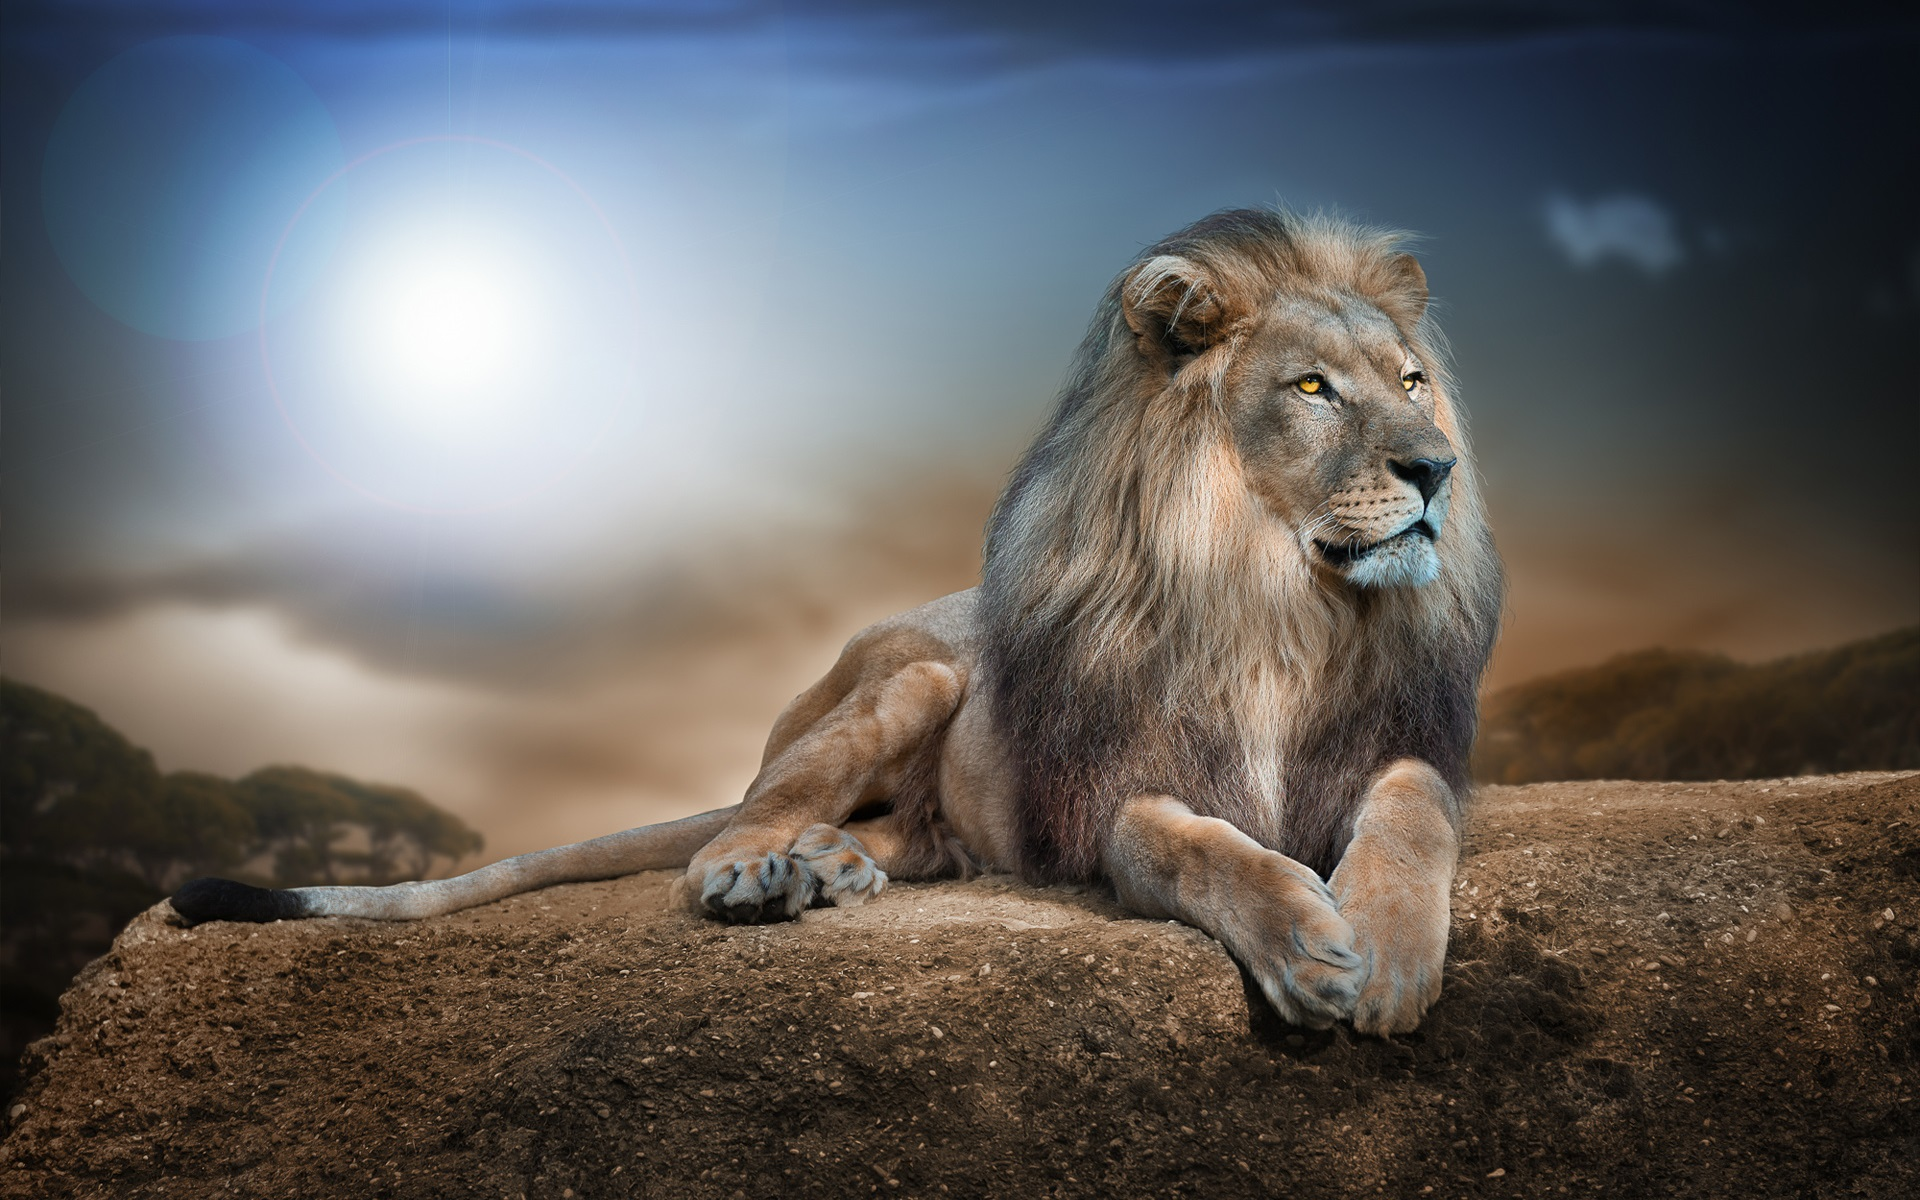
\includegraphics[width=0.5\textwidth]{./Image/figure1}
\caption{测试图}\label{Fig.figure1}
\end{figure}
}

\frame{
\frametitle{公式测试}
\[\sigma = \sin{\theta}\]
\begin{equation}
\rho = \sum_{i=0}^n{a_i}
\end{equation}
}

{\mybg
\begin{frame}[plain,noframenumbering]
 \finalpage{\yihao 感谢观看!}
\end{frame}}

\end{document}